%\documentclass{report}
%\documentclass[11pt,twoside,a4paper]{report}
\documentclass[11pt,journal,compsoc]{report}[1]
\usepackage[letterpaper, margin=0.75in]{geometry}
\usepackage{lipsum}
\usepackage{epstopdf}
\usepackage{amsthm}
\PassOptionsToPackage{hyphens}{url}
\usepackage[T1]{fontenc}
\usepackage[draft]{hyperref}
\usepackage{graphicx}
\usepackage[cmex10]{amsmath}
%\usepackage{algorithmic}
%\usepackage{algorithm}
\usepackage{array}
\usepackage{mdwmath}
\usepackage{mdwtab}
\usepackage{eqparbox}
\usepackage{ucs}
\usepackage{amsmath}
\usepackage{amsfonts}
\usepackage{amssymb}
%\usepackage{graphicx}
%\usepackage{caption}
\usepackage{url}
\usepackage{multirow}
\usepackage{hhline}
\usepackage{multicol}
\usepackage{xcolor}
\usepackage{listings}
\lstset{basicstyle=\ttfamily,
  showstringspaces=false,
  commentstyle=\color{red},
  keywordstyle=\color{blue}
}

%\definecolor{coback}{RGB}{245,245,245}
%
%\lstdefinestyle{myCustomMatlabStyle}{
%  language=c,
%  numbersep=10pt,
%  tabsize=4,
%  showspaces=false,
%  showstringspaces=false,
%  backgroundcolor=\color{coback},
%  keywordstyle=\color{black}\bfseries
%} 

\usepackage[framemethod=tikz]{mdframed}

\definecolor{light-gray}{gray}{0.95}
\lstset{basicstyle=\scriptsize\upshape\ttfamily,tabsize=4,numbersep=10pt,language=Matlab,keywordstyle=\color{black}\bfseries}

\surroundwithmdframed[
  hidealllines=true,
  backgroundcolor=light-gray,
  innerleftmargin=10pt,
  innertopmargin=0pt,
  innerbottommargin=0pt]{lstlisting}                  

\DeclareMathOperator*{\argmin}{argmin}
\DeclareMathOperator*{\argmax}{argmax}
\newcommand*{\argminl}{\argmin\limits}
\newcommand*{\argmaxl}{\argmax\limits}
\newcommand{\Am}{\mathrm{A}}
\newcommand{\Cm}{\mathrm{C}}
\newcommand{\Gm}{\mathrm{G}}
\newcommand{\Tm}{\mathrm{T}}


\usepackage[pagestyles]{titlesec}
\titleformat{\chapter}[display]{\normalfont\bfseries}{}{0pt}{\huge}
\newpagestyle{mystyle}
{\sethead[\thepage][][\chaptertitle]{}{}{\thepage}}
\pagestyle{mystyle}

%\copyrightyear{2016} \pubyear{2016}
%\access{Advance Access Publication Date: Day Month 2016}
%\appnotes{Manuscript Category}

\AtBeginDocument{\renewcommand{\abstractname}{}}
\renewcommand{\abstractname}{} 
\renewcommand{\baselinestretch}{1.3}

\begin{document}
%\firstpage{1}

\title{
%
\begin{figure}[h!]
\centerline{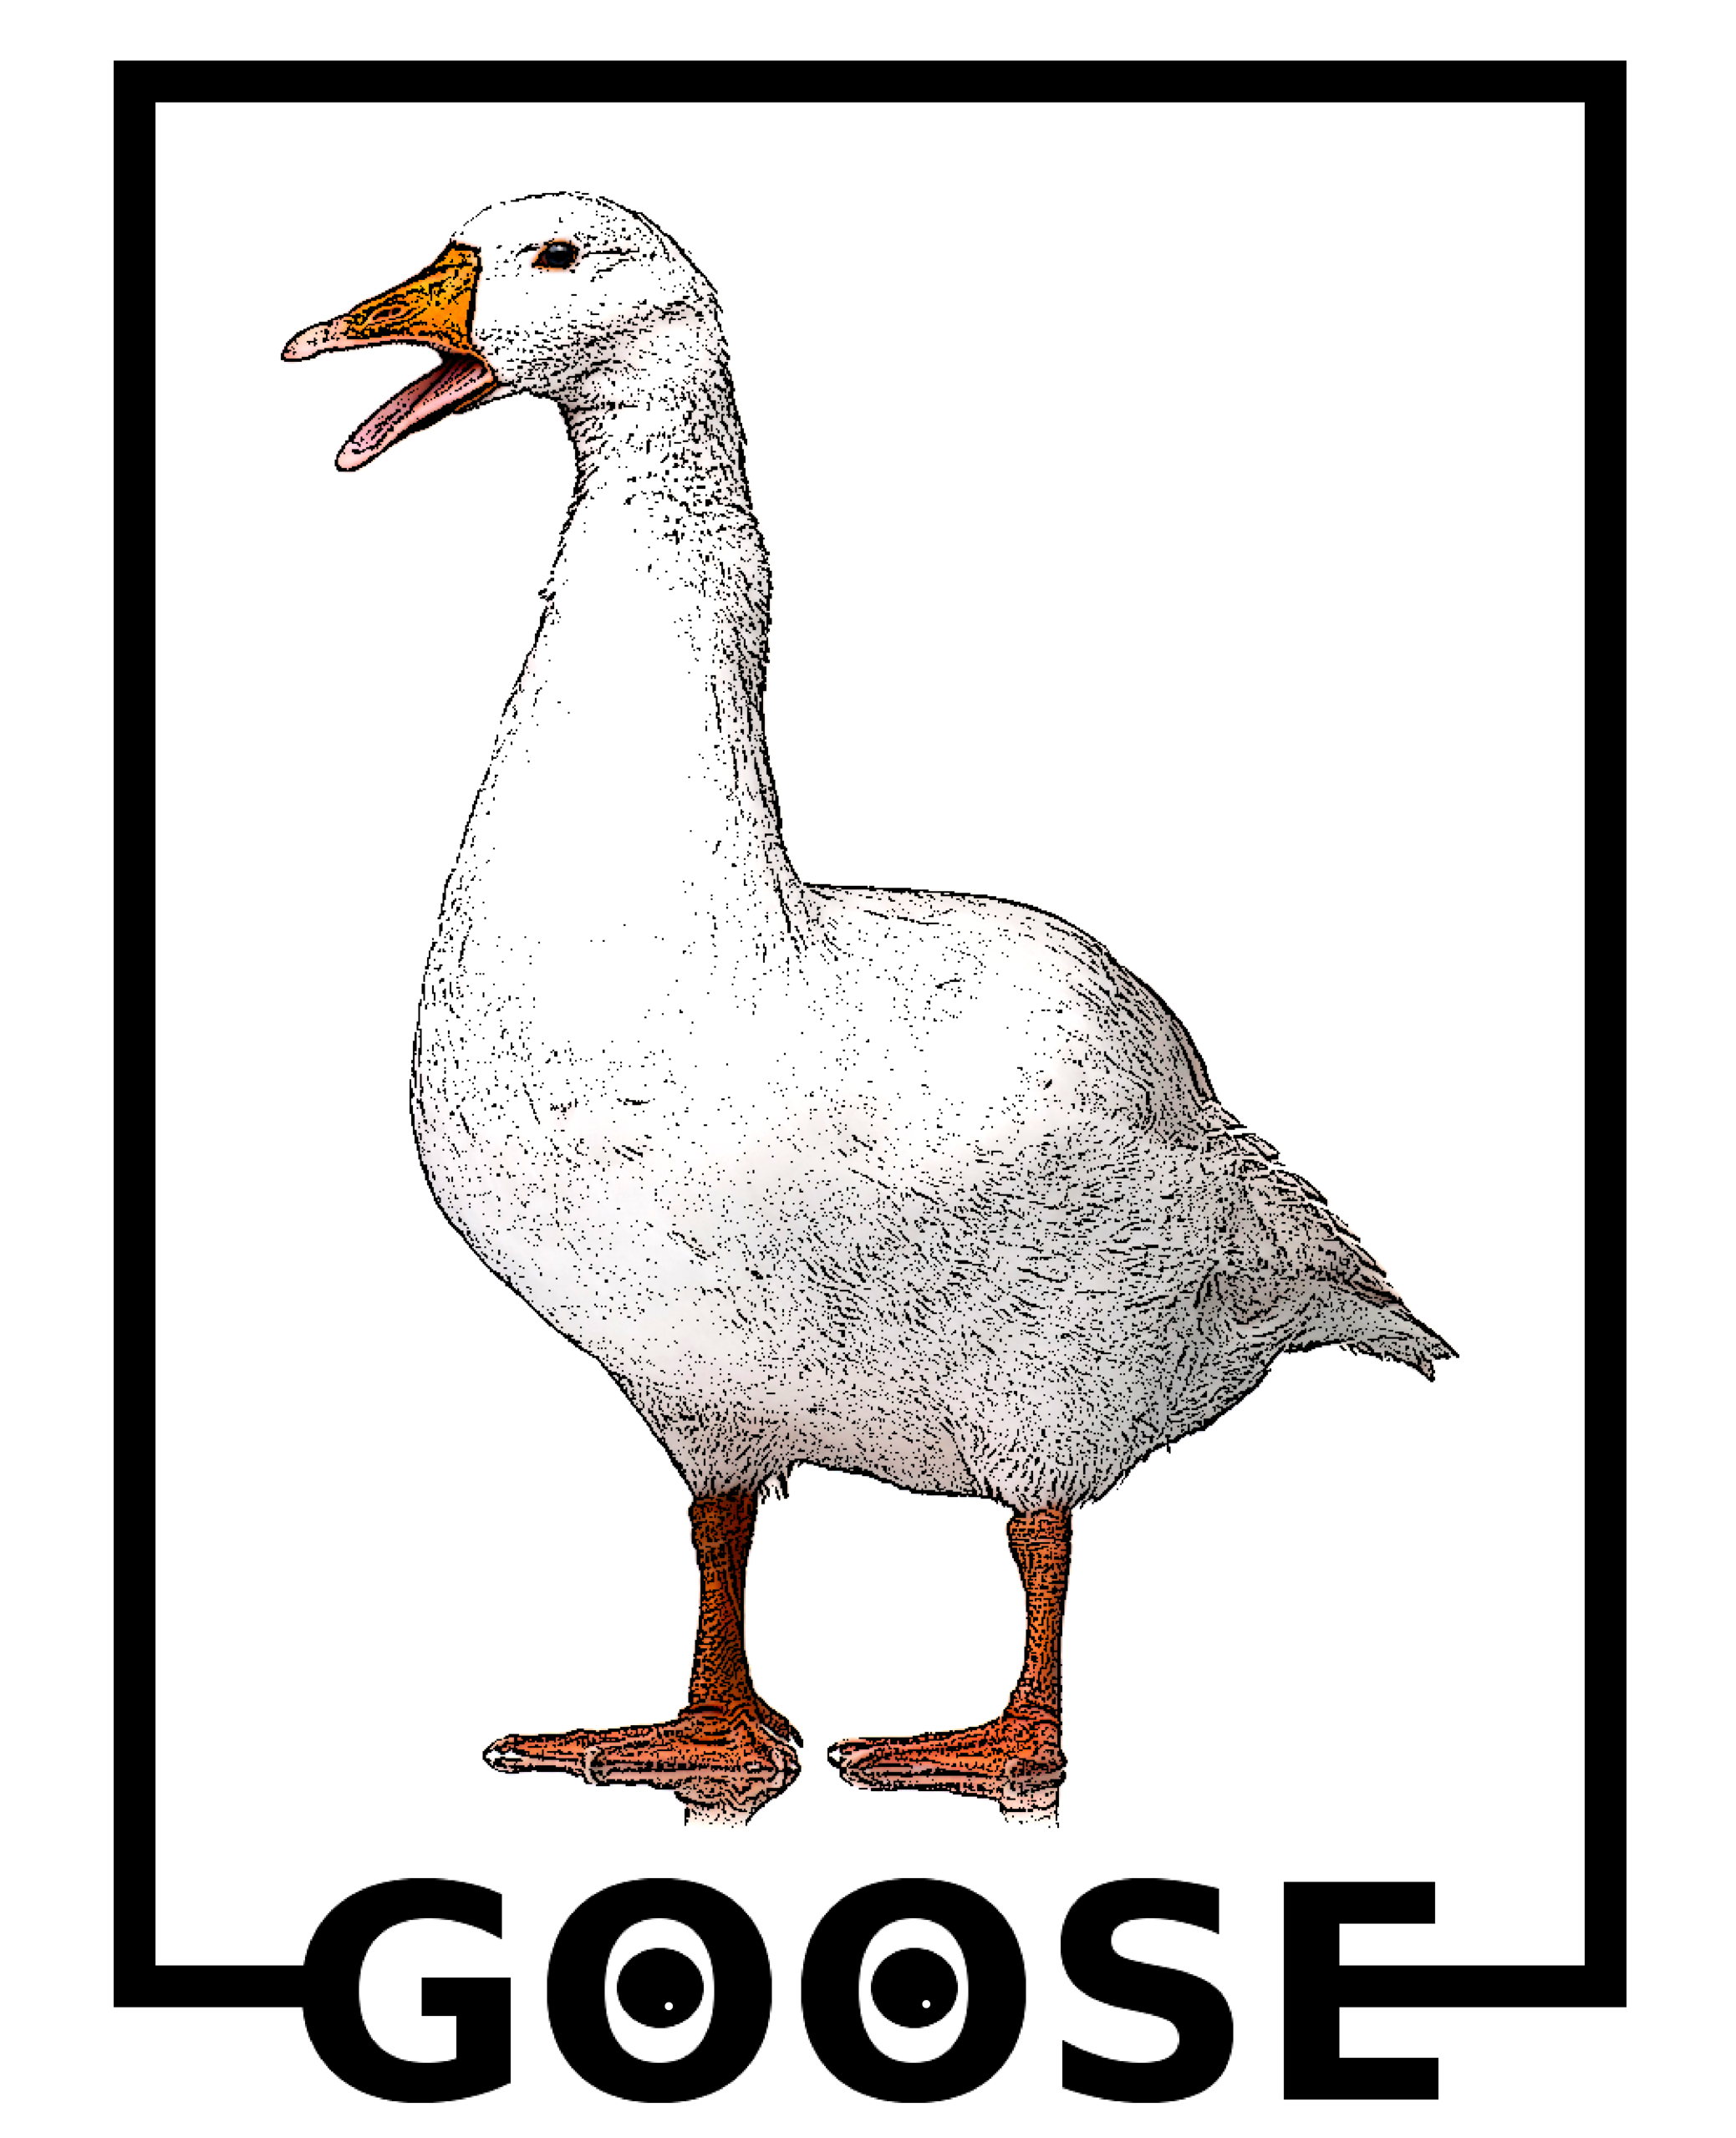
\includegraphics[width=5cm]{../imgs/logo.pdf}}
\label{logo}
\end{figure}
~\\
\textbf{A toolkit for DNA sequence\\ analysis and manipulation}
~\\~\\
\large
D. Pratas (pratas@ua.pt)\\
A. J. Pinho (ap@ua.pt)
~\\~\\
\small
IEETA/DETI, University of Aveiro, Portugal\\
}
\date{}
\maketitle

\tableofcontents

\chapter*{Simulation tools}
\addcontentsline{toc}{chapter}{Simulation tools}



%%%%%%%%%%%%%%%%%%%%%%%%%%%%%%%%%%%%%%%%%%%%%%%%%%%%%%%%%%%%%%%%%%%%%%%%%%%%%%%%
%%%%%%%%%%%%%%%%%%%%%%%%%%%%%%%%%%%%%%%%%%%%%%%%%%%%%%%%%%%%%%%%%%%%%%%%%%%%%%%%
%%%%%%%%%%%%%%%%%%%%%%%%%%%%%%%%%%%%%%%%%%%%%%%%%%%%%%%%%%%%%%%%%%%%%%%%%%%%%%%%
\chapter*{Compression tools}
\addcontentsline{toc}{chapter}{Compression tools}


%%%%%%%%%%%%%%%%%%%%%%%%%%%%%%%%%%%%%%%%%%%%%%%%%%%%%%%%%%%%%%%%%%%%%%%%%%%%%%%%
%%%%%%%%%%%%%%%%%%%%%%%%%%%%%%%%%%%%%%%%%%%%%%%%%%%%%%%%%%%%%%%%%%%%%%%%%%%%%%%%
%%%%%%%%%%%%%%%%%%%%%%%%%%%%%%%%%%%%%%%%%%%%%%%%%%%%%%%%%%%%%%%%%%%%%%%%%%%%%%%%
\chapter*{Note 11: Software availability \& characteristics}
\addcontentsline{toc}{chapter}{Note 11: Software availability \& characteristics}
\label{C-SOFTWARE}

~\\
~\\
All source code for the FALCON is available at:
\begin{itemize}
\begin{sloppypar}
\item \url{https://github.com/pratas/falcon}.
\end{sloppypar}
\end{itemize}
~\\
FALCON includes the following programs (See Note~2 for a common pipeline using 
the programs):
\begin{enumerate}
\begin{sloppypar}
\item \textbf{FALCON} - infers metagenomic composition;
\item \textbf{FALCON-FILTER} - filters local similarity of inferred sequences;
\item \textbf{FALCON-EYE} - displays the output from FALCON and FALCON-FILTER in 
a compact map;
\end{sloppypar}
\end{enumerate}

\section*{FALCON program}
\addcontentsline{toc}{section}{11.1~~~FALCON program}

The FALCON program enables to identify and quantify the similarity between
present-days reference sequences and the FASTQ reads from ancient genomes.
In the following subsections, we explain the input and output paramters.

\subsection*{Input parameters}
\addcontentsline{toc}{subsection}{11.1.1~~~Input parameters}

The FALCON program needs two files for the computation. The FILE1,
with the reads provided from the NGS platform, and the FILE2,
with the multi-FASTA cointaining the sequences of the genomes and
respective headers, are mandatory arguments. The rest of the parameters
are non mandatory, namely:
\begin{lstlisting}
Usage: FALCON [OPTION]... [FILE1] [FILE2]                                
A compression-based method to infer metagenomic sample composition.      
                                                                         
Non-mandatory arguments:                                                 
                                                                         
  -h                       give this help,                               
  -F                       force mode (overwrites top file),             
  -V                       display version number,                       
  -v                       verbose mode (more information),              
  -Z                       database local similarity,                    
  -s                       show compression levels,                      
  -l <level>               compression level [1;44],                    
  -p <sample>              subsampling (default: 1),                    
  -t <top>                 top of similarity (default: 20),              
  -n <nThreads>            number of threads (default: 2),              
  -x <FILE>                similarity top filename,                      
  -y <FILE>                local similarities filename,                  
                                                                         
Mandatory arguments:                                                     
                                                                         
  [FILE1]                  metagenomic filename (FASTA or FASTQ),        
  [FILE2]                  database filename (FASTA or Multi-FASTA).
\end{lstlisting}
There are two hidden parameters. One for setting the cache size:
\begin{lstlisting}
  -c <cache>             maximum collisions for hash cache. Memory     
                         values are higly dependent of the parameter   
                         specification.                                
\end{lstlisting}
This is a parameter that affects the precision and computational resources
needed for the computation. Lower values use less memory. For a complete
description see \cite{Pratas-2016a,Pratas-2016b}.
The previous parameter is only needed when the context of the Markov model
is higher than 13. For setting specifically the models through the command
line use the following explanation (more information can be found at 
\cite{Pratas-2016a,Pratas-2016b}):

\subsection*{Output}
\addcontentsline{toc}{subsection}{11.1.2~~~Output}

The output of the FALCON program are two files. One file contains the top-$n$ 
values with the highest similarity relatively to the reads. The following 
output shows an example of a top-5:
\begin{lstlisting}
1	9472	92.597	548558394	Human endogenous retrovirus K113
2	4668621	42.184	1069460419	Escherichia coli strain 210221272
3	4558287	42.016	1008930592	Shigella sp. PAMC 28760
4	4574246	36.661	844762407	Shigella boydii strain ATCC 9210
5	4878853	36.531	992379426	Shigella sonnei strain FDAARGOS 90
\end{lstlisting} 
These column values stand, respectively, for the ranking of higher similarity, 
the sequence size, the percentage of similarity, the global identifyer (GI) and
the name of the FASTA read (genome name).\\
~\\
The other file contains the relative local similarities and it is only 
available when FALCON runs with the ``-Z'' flag. This file is the input of
the FALCON-FILTER program that we describe next. This file is packed in 
a compact format for not increasing the substantially the storage.

\section*{FALCON-FILTER program}
\addcontentsline{toc}{section}{11.2~~~FALCON-FILTER program}

The FALCON-FILTER program enables to identify and quantify where the 
similarity between present-days reference sequences and the FASTQ reads 
from ancient genomes, below a certain threshold, occurs.
In the following subsections, we explain the input and output paramters.

\subsection*{Input parameters}
\addcontentsline{toc}{subsection}{11.2.1~~~Input parameters}

The FALCON-FILTER program needs only one file for the computation. The
file is provided from the output of the FALCON program (when the flag
``-Z'' is set on the FALCON program). The non-mandatory arguments are
mostly filters and the threshold.
\begin{lstlisting}
Usage: FALCON-FILTER [OPTION]... [FILE]                                  
Filter and segment FALCON output.                                        
                                                                         
Non-mandatory arguments:                                                 
                                                                         
  -h                       give this help,                               
  -F                       force mode (overwrites top file),             
  -V                       display version number,                       
  -v                       verbose mode (more information),              
  -s  <size>               filter window size,                           
  -w  <type>               filter window type,                           
  -x  <sampling>           filter window sampling,                       
  -sl <lower>              similarity lower bound,                       
  -su <upper>              similarity upper bound,                       
  -dl <lower>              size lower bound,                             
  -du <upper>              size upper bound,                             
  -t  <threshold>          threshold [0;2.0],                            
  -o  <FILE>               output filename,                              
                                                                         
Mandatory arguments:                                                     
                                                                         
  [FILE]                   profile filename (from FALCON).
\end{lstlisting}

\subsection*{Output}
\addcontentsline{toc}{subsection}{11.2.2~~~Output}

The output of the file contains the coordinates of the relative
similar regions with the respective self-similarity classification.

\addcontentsline{toc}{chapter}{Bibliography}
\bibliographystyle{IEEEtran}
\bibliography{defs,SPLc,SPLj,Cod,Bio,Book,Anc,Patho}

\end{document}
